\documentclass[12]{amsbook}

\usepackage{amssymb,amsmath}

%\usepackage{refcheck}
\usepackage{subcaption}
\usepackage{graphicx}
\usepackage{amssymb}
\usepackage{mathrsfs}
\usepackage{amsmath}
\usepackage{latexsym}
\usepackage{amssymb}
\usepackage{enumerate}
\usepackage{fullpage} 
\usepackage{setspace}
\usepackage{color}
%\usepackage{ dsfont }
\usepackage{float}
\usepackage{physics}
\usepackage{hyperref}

%new math symbols taking no arguments
\newcommand\0{\mathbf{0}}
\newcommand\CC{\mathbb{C}}
\newcommand\FF{\mathbb{F}}
\newcommand\NN{\mathbb{N}}
\newcommand\QQ{\mathbb{Q}}
\newcommand\RR{\mathbb{R}}
\newcommand\ZZ{\mathbb{Z}}
\newcommand\bb{\mathbf{b}}
\newcommand\kk{\Bbbk}
\newcommand\mm{\mathfrak{m}}
\newcommand\pp{\mathfrak{p}}
\newcommand\xx{\mathbf{x}}
\newcommand\yy{\mathbf{y}}
\newcommand\GL{\mathit{GL}}
\newcommand\into{\hookrightarrow}
\newcommand\nsub{\trianglelefteq}
\newcommand\onto{\twoheadrightarrow}
\newcommand\minus{\smallsetminus}
\newcommand\goesto{\rightsquigarrow}
\newcommand\nsubneq{\vartriangleleft}

%redefined math symbols taking no arguments
\newcommand\<{\langle}
\renewcommand\>{\rangle}
\renewcommand\iff{\Leftrightarrow}
\renewcommand\phi{\varphi}
\renewcommand\implies{\Rightarrow}

%new math symbols taking arguments
\newcommand\ol[1]{{\overline{#1}}}

%redefined math symbols taking arguments
\renewcommand\mod[1]{\ (\mathrm{mod}\ #1)}

%roman font math operators
\DeclareMathOperator\aut{Aut}

%for easy 2 x 2 matrices
\newcommand\twobytwo[1]{\left[\begin{array}{@{}cc@{}}#1\end{array}\right]}

%for easy column vectors of size 2
\newcommand\tworow[1]{\left[\begin{array}{@{}c@{}}#1\end{array}\right]}

\newtheorem{theorem}{Theorem}[section]
\newtheorem{corollary}{Corollary}[theorem]
\newtheorem{lemma}[theorem]{Lemma}
\newtheorem{exercise}[theorem]{Exercise}
\newtheorem{definition}[theorem]{Definition}

\title{PHY 365L Final Project: Neural Circuits}
\author{Faris Sbahi}


\begin{document}
\maketitle

\begin{abstract}
In this project, we construct and study circuits which are meant to model the actions potentials of several classes of neurons. We aim to understand the fundamentals of electronics in addition to those of cell and molecular biology of nerve cells.
\end{abstract}

\chapter{Neurons and Axons}

\section{Introduction}

\subsection{Overview}

The essence of nervous system function is signaling, or transferring information. Signaling is essential for an organism to (1) sense information about its environment, (2) import this information into its brain where it can be processed, and (3) generate a behavioral response.

\subsection{Mathematical Modeling}

Alan Lloyd Hodgkin and Andrew Huxley, in 1963, won the Nobel Prize in Physiology and Medicine for their work developing the Hodgkin-Huxley (H-H) Equations, equations that modeled to incredible accuracy the propagation of action potentials through a squid axon. 

In our project, we seek to captre the important qualitative behaviors of the axon system using electronics. Before speaking of electronics, it is prudent to develop differential equations which simplify the H-H model.

The Hodgkin-Huxley model models the cell membrane as a simple circuit. 

\begin{figure}[h]
    \centering
    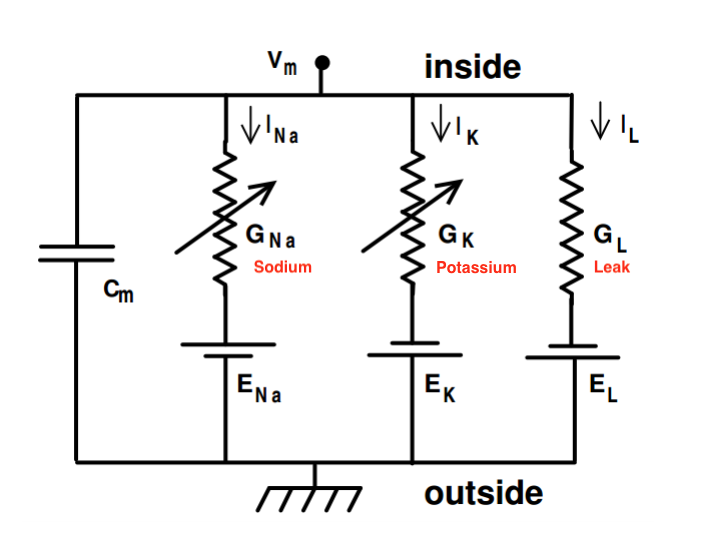
\includegraphics[scale=0.5]{hhmodel}
    \caption{Hodgkin-Huxley Circuit}
    \label{fig:my_label}
\end{figure}

Two voltage-dependent sodium and potassium channels allow the ions to flow through the membrane. The membrane has a capacitance indicated by $c_m$. Additionally, the sodium and potassium channels have a conductance parameter $G_{Na}$ and $G_K$, as well as a leakage conductance as shown. These conductance parameters can be modeled by various functions as will be shown later, and model the buildup in the passage of ions that create the action potential. The circuit is in parallel to mimic the axon. 

Using classic current conservation in a circuit, and adding the parameter of an external current $I_{ext}$, we can derive the current equation for the cell.

\begin{align*}
    c_m\frac{dV_m}{dt} + I_{ion} = I_{ext}
\end{align*}

In our particular model, we will assume that $G_L$ is constant and the capacitance $c_m$ as well. $V_m$ is the potential within the cell membrane, and $I_{ion}$ is the net ionic current within the cell.

The derivation of each ionic current through the different channels depends on the conductance parameter times the driving potential.

\begin{align*}
    I_{ion} = G_{ion}(V_{m}-E_{ion})
\end{align*}

The physical meaning of conductance is the probability that the channels that the ions pass through will be considered open, or when the gates that the ions can pass through are all permissive in that particular ion channel. This is dependent on the voltage of the cell membrane. 

Hodgkin and Huxley used three different types of gates to model the conductance channels. Using, $m$, $h$, and $n$ as different types of gates (iterations of $p$), $G_{Na}$ and $G_K$ are modeled as followed.

\begin{align*}
    G_{Na} &= \bar{G}_{Na}m^3h\\
    G_{K} &= \bar{G}_{K}n^4
\end{align*}

Where $m$, $h$, and $n$ follow the following differential equation, which is derived on the open fraction of gates, $p$:

\begin{align}
\label{eq:dpdt}
    \frac{dp}{dt} = a(V)(1-p) - b(V)p
\end{align}

Hodgkin and Huxley discovered that as they kept the voltage constant, the conductance of the channels increased steadily to a maximum value. They used this experimental data to achieve equations for the time step of increase of $p$.

\begin{align}
\label{eq:time}
    p_{\infty}(V) &= \frac{a_p(V)}{a_p(V) + b_p(V)} \\
    \tau_p(V) &= \frac{1}{a_p(V) + b_p(V)} 
\end{align}

Where $p_{\infty}(V)$ is the steady state value at an given voltage and ${\tau_p}(V)$ are time constants of response of the gates, in relation to $p$ growing to its steady state value. These constants can be experimentally fit to data and using Equation (\ref{eq:dpdt}) we can find $a_p(V)$ and $b_p(V)$. Thus, the final equations for the rate constants are as follows:

\begin{align*}
    a_m(V) &= \frac{0.1(25-V)}{\exp(\frac{25-V}{10})-1}
    &b_m(V) = 4e^{-V/18} \\
    a_n(V) &= \frac{0.01(10-V)}{\exp(\frac{10-V}{10})-1} 
    &b_n(V) = 0.125e^{\frac{-V}{80}}\\
    a_h(V) &= 0.07e^{\frac{-V}{20}} 
    &b_h(V) = \frac{1}{\frac{\exp(30-V)}{10}+1}
\end{align*}

We can also simplify equation (\ref{eq:dpdt}) to the following.

\begin{align*}
    \frac{dp}{dt} = \frac{p_{\infty}(V)-p}{\tau_p(V)}
\end{align*}

The combined system of differential equations is shown in the next section. Furthermore, in Figure \ref{fig:inf} we show the values of $m_\infty$ and $n_\infty$ derived using the equations above. 

\begin{figure}
\centering
	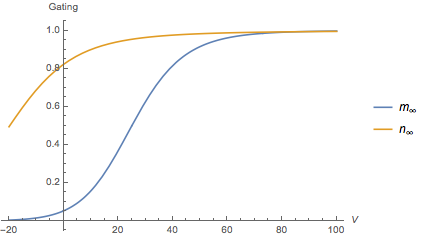
\includegraphics[height=5cm]{gating.png}
	\caption{$m_{\infty}$ (blue) and $n_{\infty}$ (orange)}
		\label{fig:inf}
\end{figure}

\subsection{Circuit Modeling} 

Maeda and Makino \cite{maeda2000pulse} show how to model a neuron using 3 transistors for a FitzHugh-Nagumo type neuron. In the FitzHugh-Nagumo model, one simplifies the Hodgkin-Huxley formulation by replacing the fast Na current of the H-H model with a simplified fast, depolarizing, activation process. Furthermore, one replaces the slow $Na$ inactivation and slow, repolarizing, $K$ current by a single slow inactivation process. By adding one more repolarizing process, modeled by two more transistors, they can produce a neuron with bursting behavior. 

Evidently, the state variables for the model are $V$, $m$, $h$, and $n$. Hence, we can write

\begin{align*}
    C\frac{dV}{dt} &= I_{ext} -\bar{G}_{Na}m^3h(V-E_{Na}) -\bar{G}_{K}n^4(V-E_{K})  -\bar{G}_{L}m^3h(V-E_{L}) \\
    \frac{dm}{dt} &= \frac{m_{\infty}(V)-m}{\tau_m(V)} \\
    \frac{dh}{dt} &= \frac{h_{\infty}(V)-h}{\tau_h(V)} \\
    \frac{dn}{dt} &= \frac{n_{\infty}(V)-n}{\tau_n(V)} 
\end{align*}

While analyzing a four-dimensional nonlinear system is certainly feasible, it is difficult to then visualize our results. Furthermore, the number of combinations of parameters grows exponentially with each new parameter introduced.

\begin{figure}[h]
\centering
\begin{subfigure}{.5\textwidth}
	\centering
	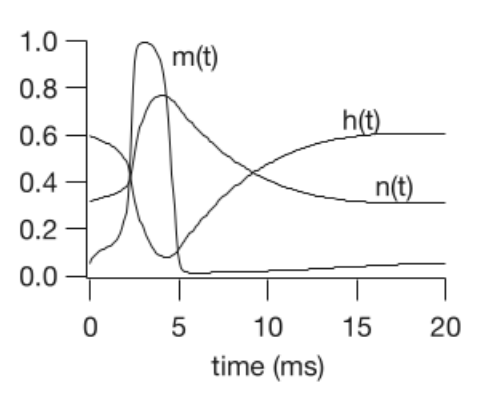
\includegraphics[height=5cm]{keener1.png}
	\caption{Gate Variables}
\end{subfigure}%
\begin{subfigure}{.5\textwidth}
	\centering
	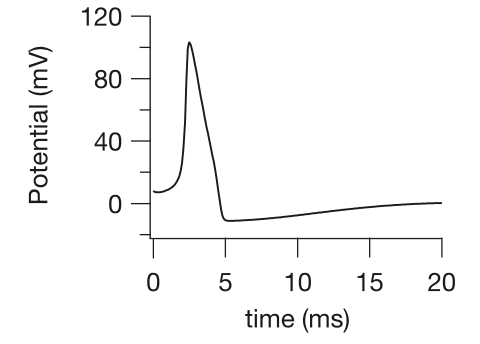
\includegraphics[height=5cm]{keener2.png}
	\caption{Action Potential}
\end{subfigure}
	\caption{Dynamics of H-H model Without Approximation on Shared Time-Scale (ms)}
	\label{fig:keen}
\end{figure}


From Equation \ref{eq:time}, it's clear that the time constants, $\tau_i$ vary widely between these equations. For example, for a 20 mV potential, the values are $\tau_m \approx 0.4 ms$, $\tau_h \approx 8 ms$, and $\tau_n \approx 5 ms$. In general, it is true that $\tau_m$ is much smaller than the other time constants. Recall that $\tau_m$ is a measure of the speed with which $m$ converges to its steady state value $m_\infty$. Therefore, it may be a reasonable assumption to assume that $\tau_m$ is so fast compared to the other parameters that $m = m_\infty$. Then, we can either take $n$ or $h$ to be constant which would then give us a two-dimensional nonlinear system. Since $h$ fluctuates over the largest time-scale, we'll take it to be some constant $\bar{h}$. As a result, we have 

\begin{align*}
        C\frac{dV}{dt} &= I_{ext} -\bar{G}_{Na}m_\infty^3\bar{h}(V-E_{Na}) -\bar{G}_{K}n^4(V-E_{K})  -\bar{G}_{L}(V-E_{L}) \\
    \frac{dn}{dt} &= \frac{n_{\infty}-n}{\tau_n} 
\end{align*}

The assumption of taking $h$ to be constant can be judged visually in Figure \ref{fig:keen}, borrowed from Keener and Sneyd, which shows values of the unapproximated model\cite{keener}.

\begin{figure}
\centering
\begin{subfigure}{\textwidth}
	\centering
	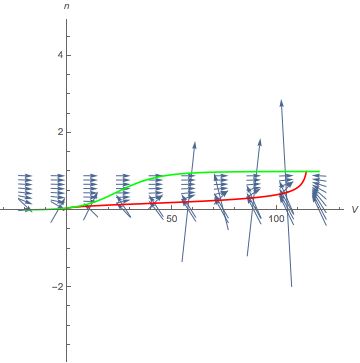
\includegraphics[width=10cm]{fastFast_nullc.png}
	\caption{$I_{ext}=0$ nullclines}
\end{subfigure}
\begin{subfigure}{\textwidth}
	\centering
	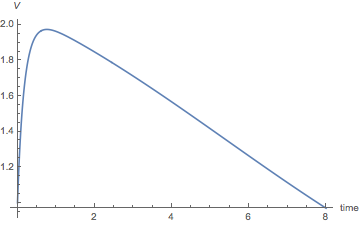
\includegraphics[width=10cm]{fastFast.png}
	\caption{$I_{ext}=0$ action potential}
\end{subfigure}
	\caption{V-nullcline (Red) and n-nullcline (Green) for $I_{ext}$ on and off of simple constant $h$ model, with associated action potentials}
	\label{fig:first}
\end{figure}

In Figure \ref{fig:first}, we see the result of the Fitzhugh-Nagumo approximation. We can see that there are three potential intersections of the nullclines (two are present in the bottom left but difficult to visualize due to their close proximity), implying that there are excited and relaxed fixed points. If one looks closely at the vector field, the excited equilibrium (upper-right) appears to be attracting, and in the lower-left one equilibrium seems to be attracting while the other is a saddle. We'll call the one that is attracting in the lower-left the rest equilibrium, since it should correspond to the action potential going to rest. We also see that the action potential looks qualitatively different than it does in the unsimplified H-H model. The model seems less than ideal, but is a good initial step. 

We could treat $n$ and $h$ as bifurcation parameters. For example, we can use our physical intuition to consider the effects of increasing $n$ and decreasing $h$. Evidently, increasing $n$ corresponds to activation of K$^+$ conductance and deactivation of Na$^+$ conductance. As a result, we could predict the disappearance of the fixed point that corresponds to an excited state. Indeed, one can show that there is a saddle node bifurcation in this scenario resulting in the disappearance of the saddle and excited fixed points.\cite{keener}.

The neurons we construct in this project follow from this approximation.

\section{Circuit 1: A Pulse Type Neuron}
 
 We begin by considering a circuit with the following structure
 
\begin{figure}[H]
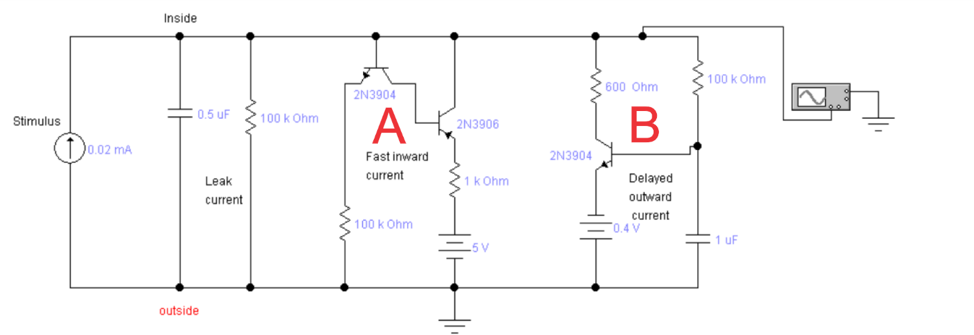
\includegraphics[width=0.8\textwidth]{exercise1-0}
\caption{"A pulse type neuron model" from \cite{maeda2000pulse}}
\end{figure}

In our experiment, instead of applying a constant current source we added a $200k\Omega$ resistor above the $5V$ voltage source. Nevertheless, the analysis follows similarly.

Hence, we consider transistor sub-circuits A and B as ideal switches. When we just turn on the current source, the upper node voltage is equal to 0. Both switches are off, and the circuit could be reduced to the following circuit
 
 \begin{figure}[H]
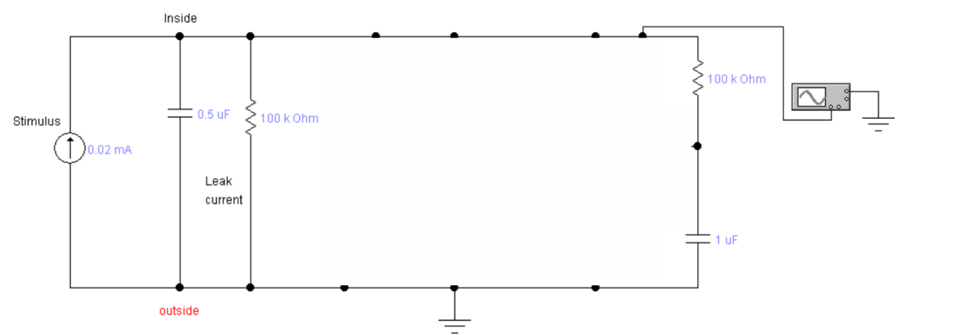
\includegraphics[width=0.8\textwidth]{exercise1-1}
\end{figure}

The dynamic of the upper node $V(t)$ depends on the values of capacitors and resistors, but the final (equilibrium) voltage depends only on the stimulus current $I$ and leak current resistor. If we are not interested in dynamics of $V(t)$, but only in its equilibrium value, we can remove capacitors from the circuit.
 
 \begin{figure}[H]
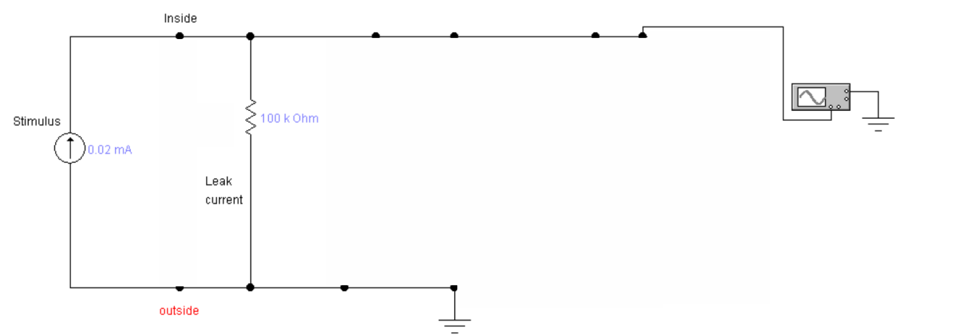
\includegraphics[width=0.8\textwidth]{exercise1-2}
\end{figure}

Clearly, we then have a current divider. Hence, the voltage is given by 

\begin{align*}
\Big(\frac{100(100)}{100 + 100}k\Omega\Big) (0.02 mA) = 	1 V
\end{align*}


Now let's turn on switch $A$
 
 \begin{figure}[H]
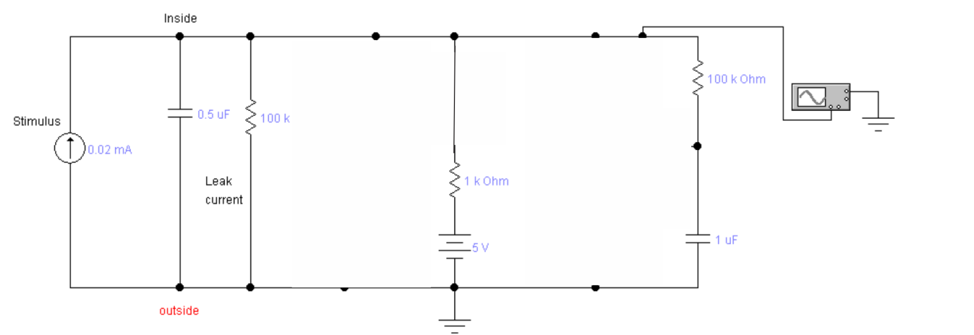
\includegraphics[width=0.8\textwidth]{exercise1-3}
\end{figure}

If we again are not interested in dynamics of V(t), we can redraw the circuit dropping all capacitors
 
 \begin{figure}[H]
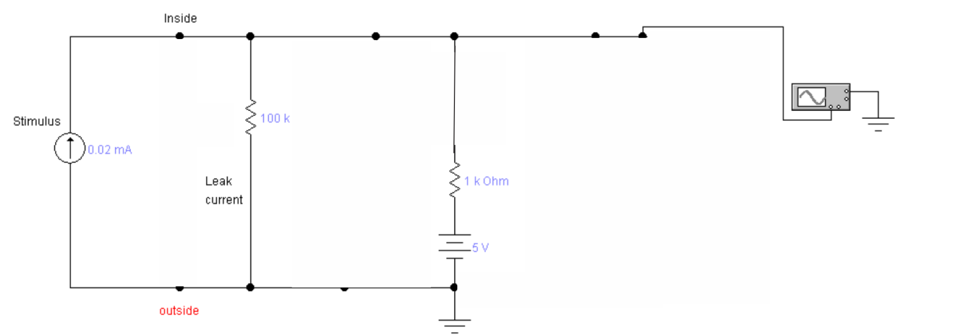
\includegraphics[width=0.8\textwidth]{exercise1-4}
\end{figure}

To find the voltage at the top node, we simply use the method of Thevenin's equivalent circuit\cite{fortney1987principles}. To calculate the Thevenin equivalent voltage, we may open all current sources and calculate the voltage at the top node. In which case, we find that we have a voltage divider which gives 

$$\frac{100}{1+100} * 5V = 4.95 V$$

Now, let's turn on the switch $B$
 
 \begin{figure}[H]
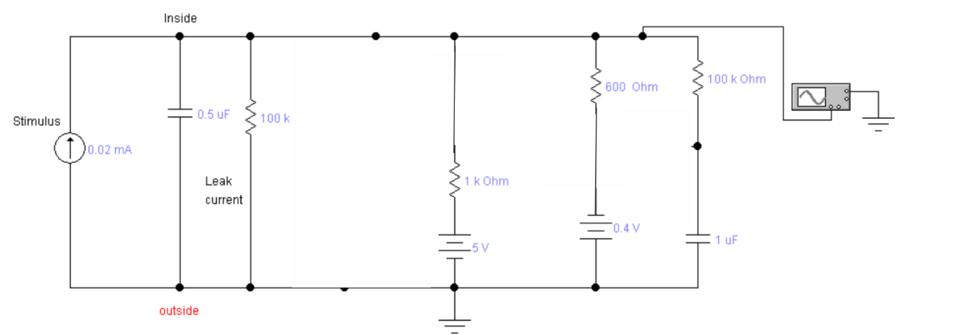
\includegraphics[width=0.5\textwidth]{exercise1-5}
\end{figure}

and drop all capacitors again
 
\begin{figure}[H]
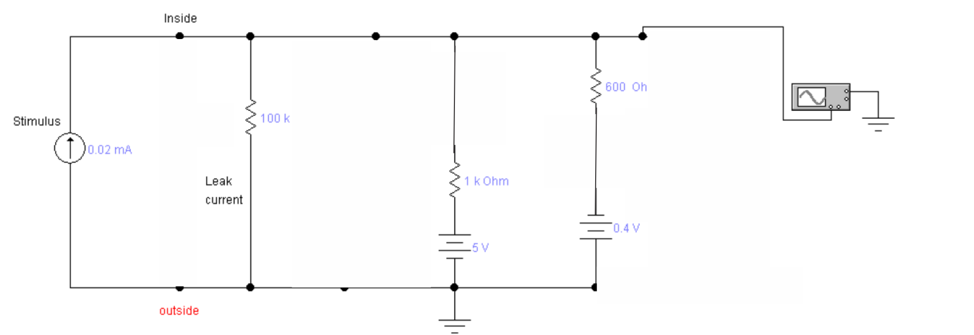
\includegraphics[width=0.5\textwidth]{exercise1-6}
\end{figure}

Find the voltage at the top node for this circuit.

\begin{figure}[H]
\centering
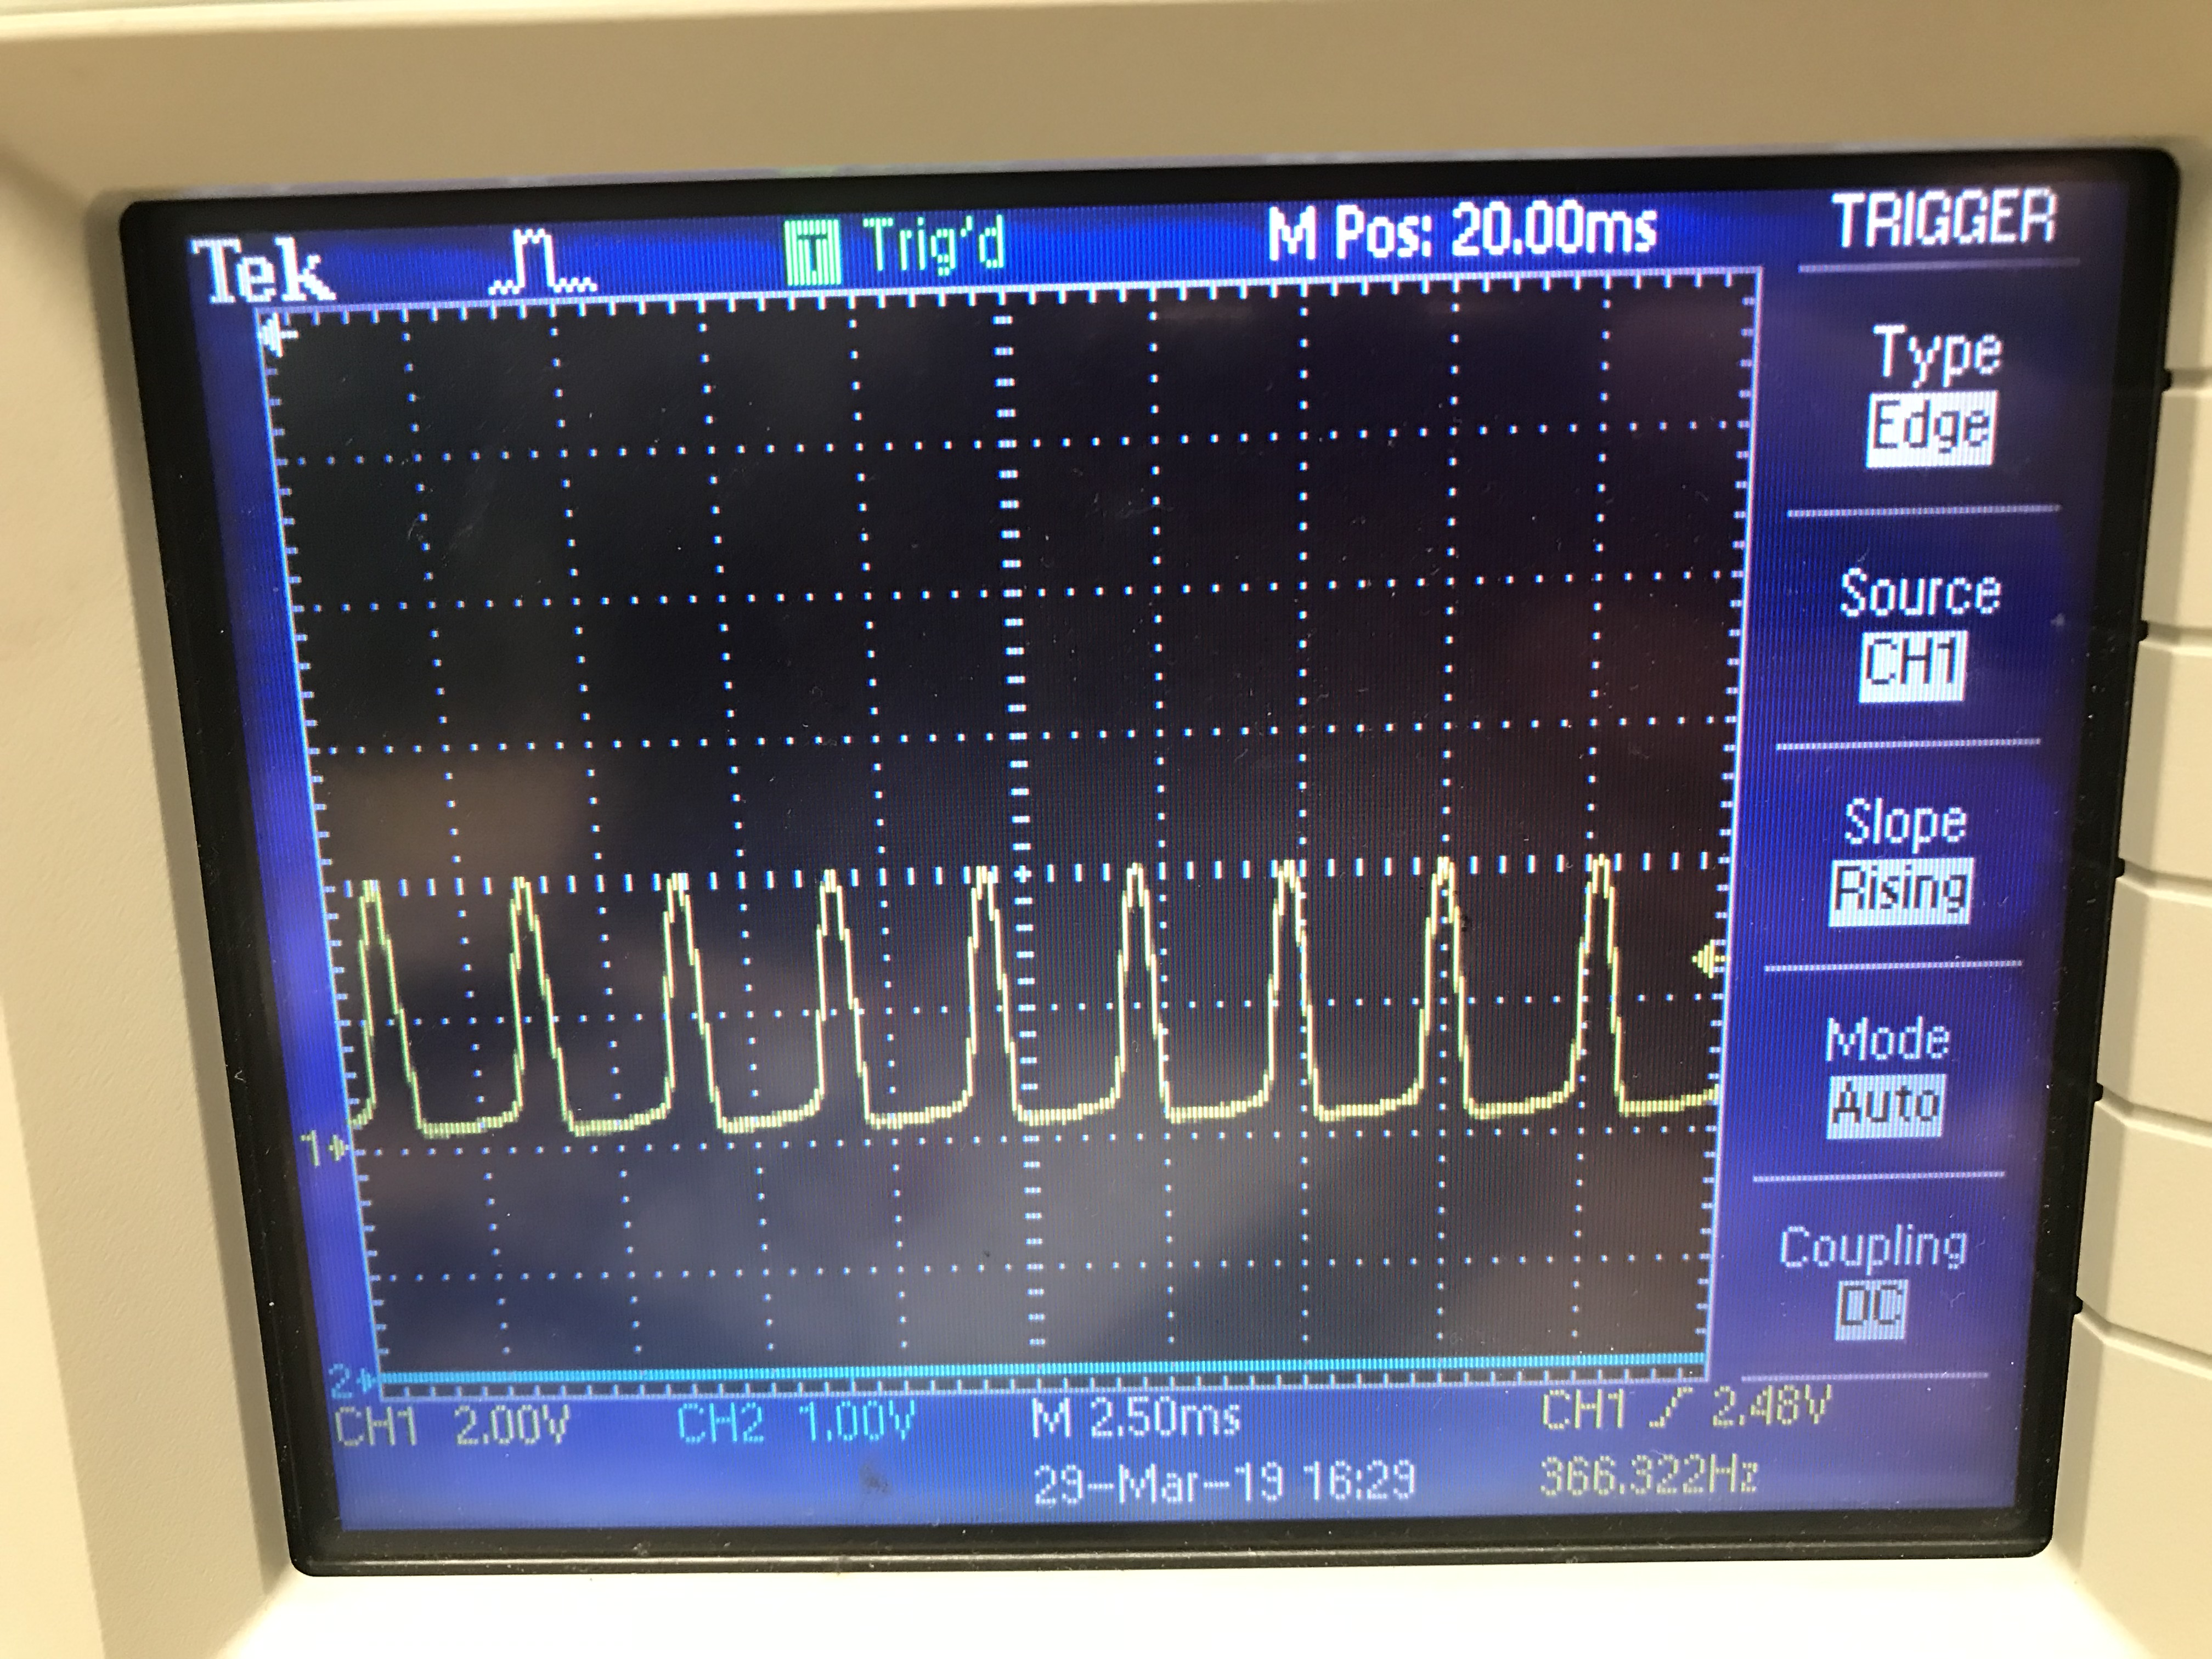
\includegraphics[width=0.7\textwidth]{neuron.jpeg}	
\end{figure}


\section{Circuit 2: A Pulse Type Neuron with Burst}

We've discussed that action potentials are fundamental to a neuron's ability to transfer information. However, there are additional aspects of its electrical properties which shape neuronal input and output. For example, some neurons that fire spontaneously in the absence of external simulation do not fire at regular intervals, but instead generate bursts of action potentials that are separated by the hyperpolarizations of the membrane. Such cells are terms "bursting" neurons \cite{levitan2015neuron}.

These bursts are used in at least two known ways \cite{levitan2015neuron}:

\begin{enumerate}
\item To generate rhythmic behaviors. For example, breathing, walking, swimming, and chewing food.	
\item To secrete neurohormones. For example, neurons located in the hypothalamic region of the mammalian brain individually contain either vasopressin or oxyocin. These hormones control water retention and lactation, respectively. Interestingly, it appears that the bursting pattern is more effective than a steady pacing pattern of firing as a stimulus to the intracellular mechanism which generates peptide release.
\end{enumerate}
 

\begin{figure}[H]
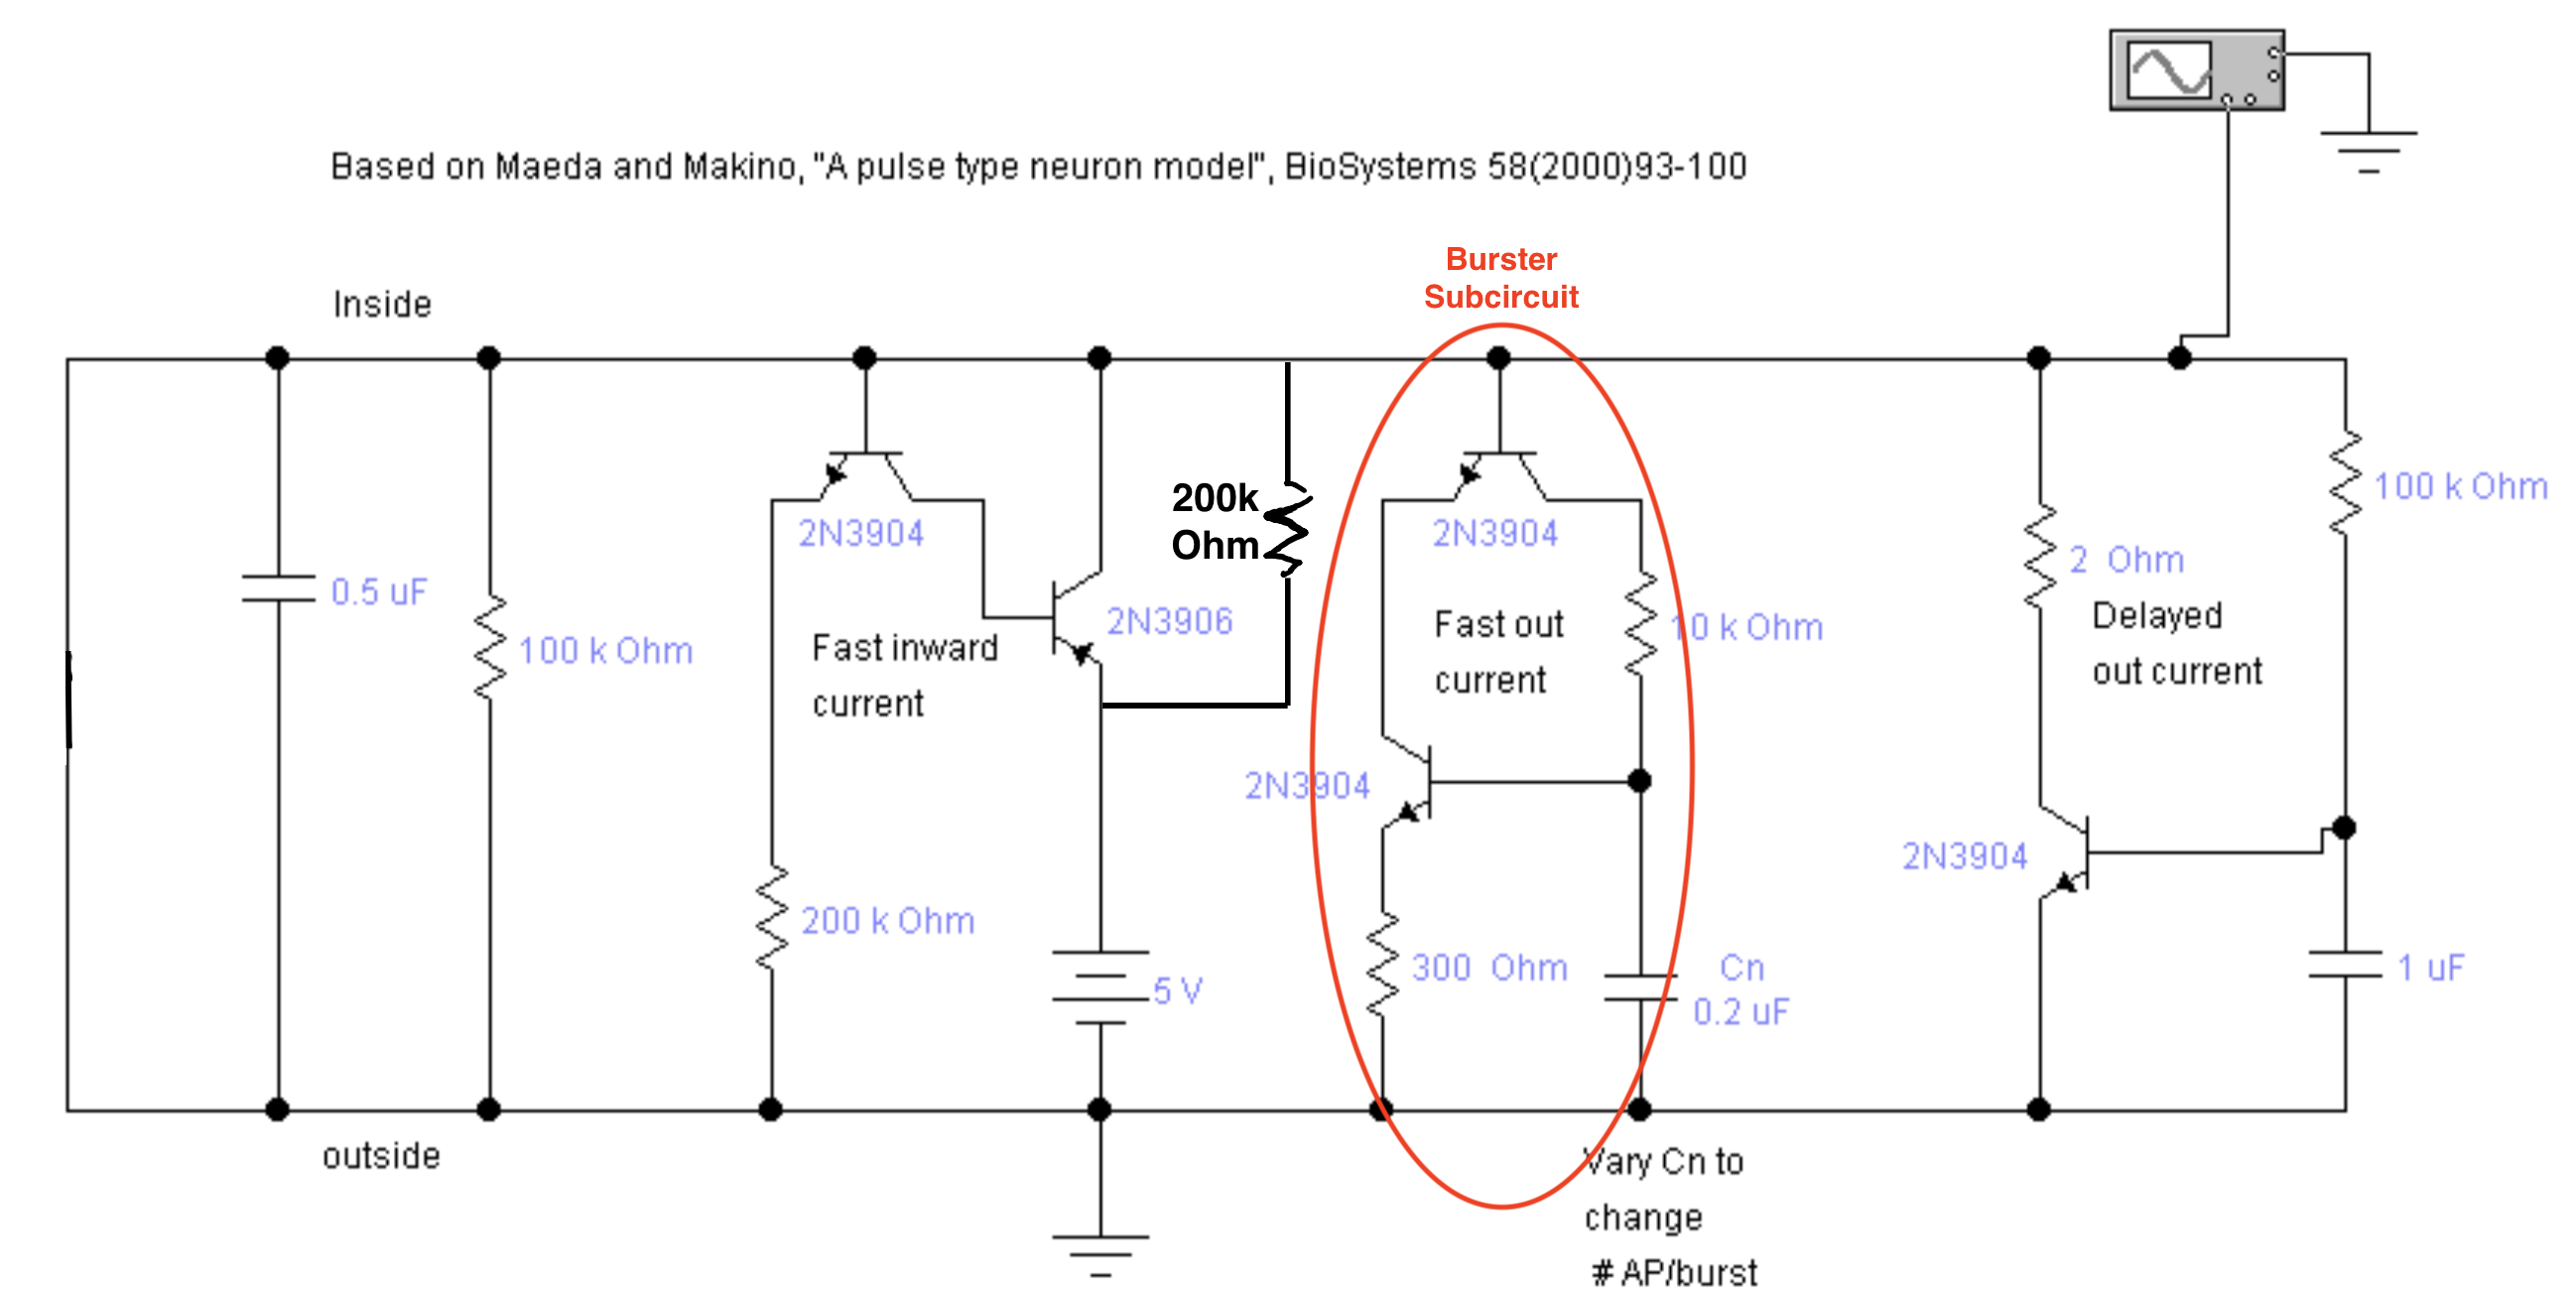
\includegraphics[width=0.7\textwidth]{burster_heart_cell}	
\end{figure}

\begin{figure}[H]
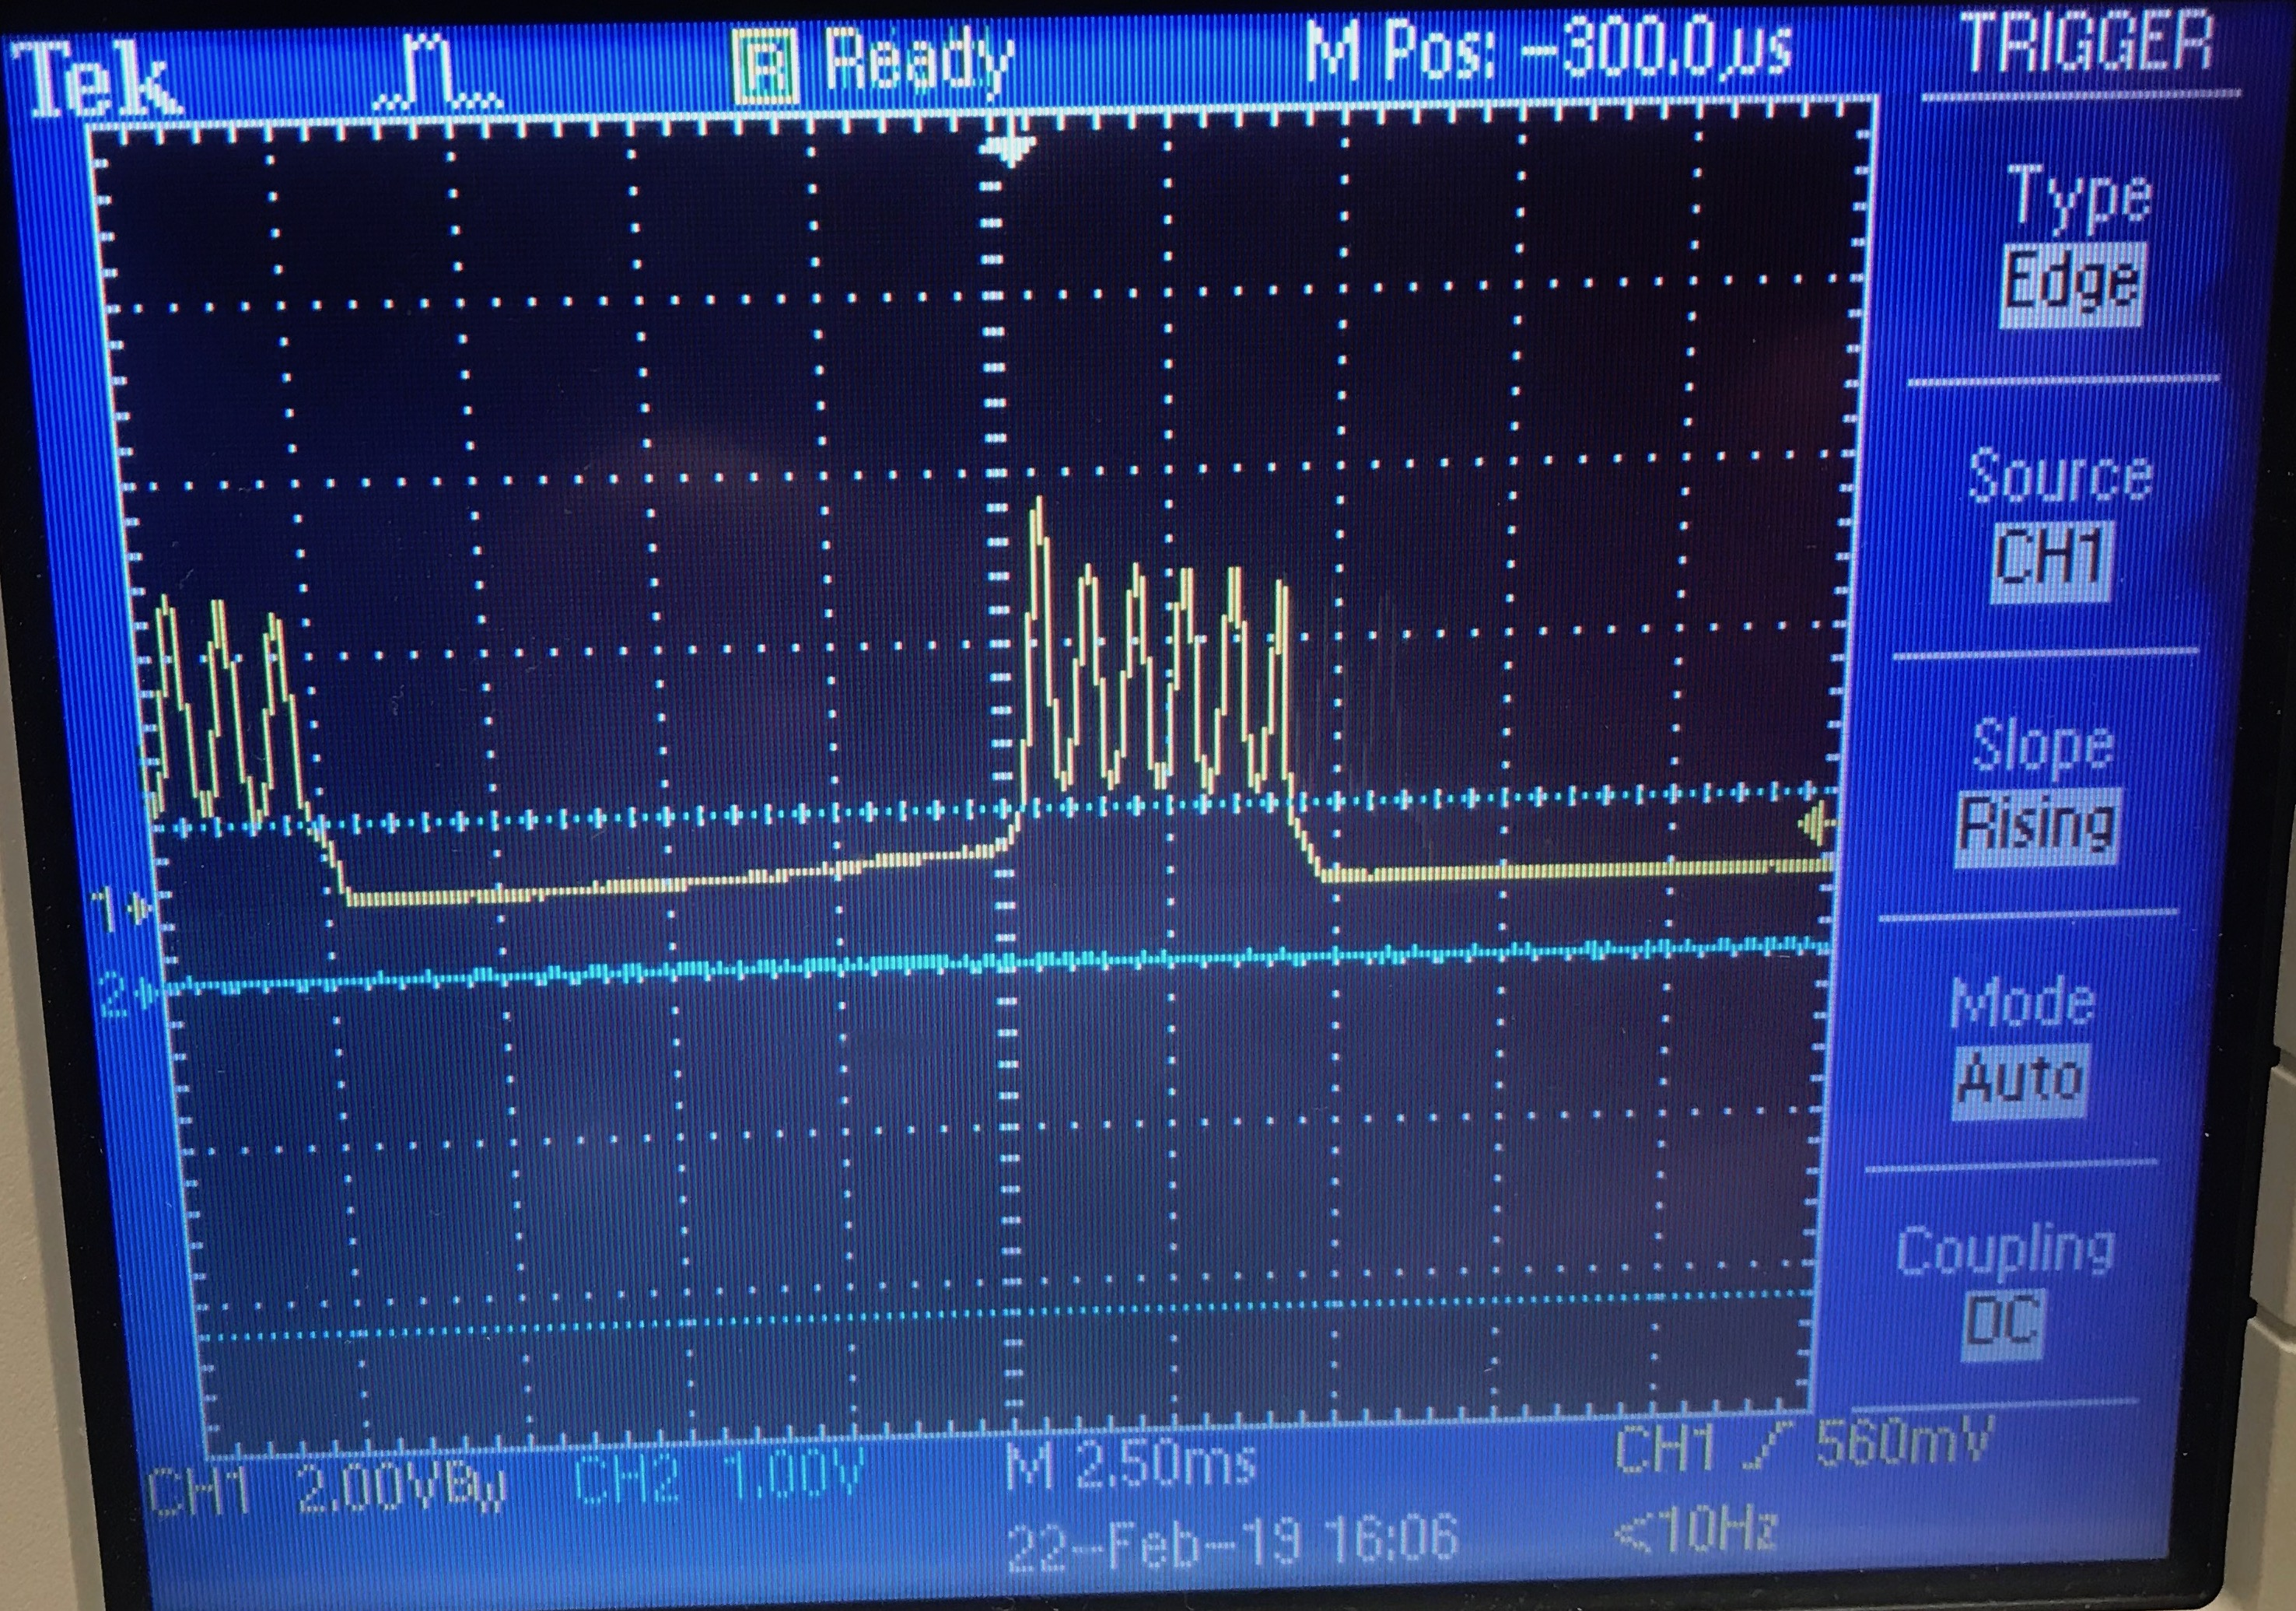
\includegraphics[width=0.5\textwidth]{burster_osc}	
\end{figure}

\chapter{Synapses}

\section{Circuit 1: Excitatory Synapse}

\begin{figure}[H]
\centering
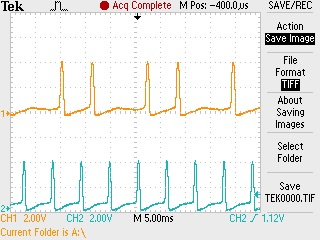
\includegraphics[width=0.5\textwidth]{excitatory.jpg}	
\end{figure}

\section{Circuit 2: Inhibitory Synapse}

\begin{figure}[H]
\centering
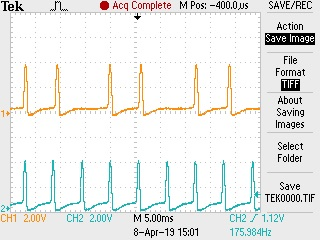
\includegraphics[width=0.5\textwidth]{inhibitory.jpg}	
\end{figure}

\chapter{}


\bibliography{phy365.bib}
\bibliographystyle{plain}
\nocite{*}


\end{document}
